\documentclass[a4paper, 12pt]{exam}
\usepackage[T1]{fontenc} 
\usepackage{amsmath}
\usepackage{amssymb}
\usepackage{enumerate}
\usepackage{bm}
\usepackage{advdate}
\usepackage{datetime}
\usepackage{graphicx}
\usepackage[mathcal]{eucal}
\usepackage{dsfont}
\usepackage[numbered,framed]{matlab-prettifier}
\usepackage[noend]{algpseudocode}
\usepackage{algorithmicx,algorithm}

\usepackage{url}
\newdate{issuedate}{25}{9}{2020}
\newdate{duedate}{9}{10}{2020}

% \newcommand{\duedate}[1][14]{%
% \begingroup
% \AdvanceDate[#1]%
% \today%
% \endgroup
% }%

\usepackage[thehwcnt=4]{iidef}
\thecourseinstitute{Tsinghua-Berkeley Shenzhen Institute}
\thecoursename{Learning From Data}
\theterm{Fall 2020}
\makeatletter
\newcommand{\firstblock}{programming_policies}
\makeatother

\begin{document}
	
	\pagestyle{headandfoot}
	\runningheadrule
	
	
	\newcounter{psctr}
	\setcounter{psctr}{4} % set to the times of problem
	
	\runningheader{Programming Assignment \thepsctr}
	{\textsc{Learning from Data}}
	{ Page \thepage\ of \numpages}
	\firstpagefooter{}{}{}
	\runningfooter{}{}{}
	
	
	\newcounter{Sequ}
	\newenvironment{Sequation}
	{\stepcounter{Sequ}%
		\addtocounter{equation}{-1}%
		\renewcommand\theequation{S\arabic{Sequ}}\equation}
	{\endequation}
	%\topskip0pt
	
	% \vspace*{\fill}
	\centering
	
	% \vspace{0.3em}
	\centering
	\renewcommand{\thequestion}{\arabic{psctr}.\arabic{question}}
	\hwname{Programming Assignment}
	\courseheader
	\begin{flushleft}
		\textbf{Issued:} \displaydate{issuedate} \hfill
		\textbf{Due:} \displaydate{duedate} 
	\end{flushleft}
	
	\hrule 
	
	\input{\firstblock}
	
	%\pointname{}
	%\vspace{\footskip}
	\vspace{1em}
	
	
	%\pointname{}
	%\vspace{\footskip}
	%\vspace{1em}
	
	\begin{questions}
		\question (5 points) \emph{maze.} Suppose there is a mouse who is hungry, thereby plans to take an exploration. An example of the \emph{Reward Matrix} it confronts is illustrated in Fig.\ref{fig1} where the blue squares are rat traps, and the red squares are cheese. 
	\begin{figure}[htbp]
\centering
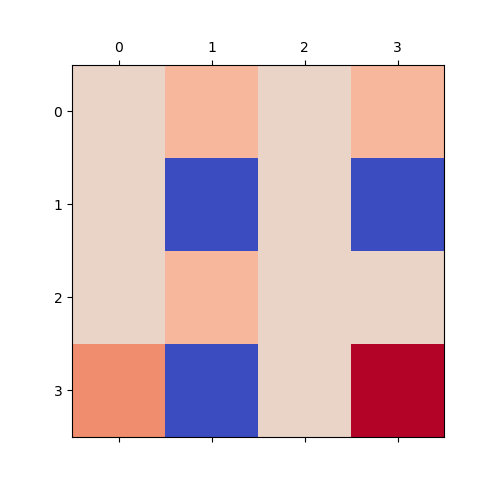
\includegraphics[width=3in]{0.png}
\caption{Reward result.}\label{fig1}
\end{figure}
 \textbf{There are several rules need to be noted}:
\begin{enumerate}[label=\roman*.]
\item The mouse at most has \textbf{4} alternative actions: left, rigth, up, down, and when it is at the boundary of the grid, it cannot jump out of it.

\item The terminal condition for learning at each step is that the mouse succeeds to eat the largest cheese (reward = 4) or the mouse is trapped (reward = -5).

\item The termination condition is either the mouse got the cheese or it is trapped.

\end{enumerate}


Now we are ought to help it learn the maze problem by value iteration.
\begin{algorithm}[H] 
\caption{MDP value iteration\label{vi}} %算法的名字
\hspace*{0.02in} {\bf Input:} %算法的输入
reward matrix $R$ and the transition probability $P_{sa}(s') = P(S_{t+1}=s'|S_t=s, a)$

\hspace*{0.02in}
{\bf Output: } value function $V$ and policy $\pi$
for each state
\begin{algorithmic}[1]
\State Initialize $V(s)=$ for each state $s$
\While{not convergent}
\For{each state $s$}
\State $V(s) = R(s) + \gamma \max_{a\in A}\sum_{s'\in S}P_{sa}(s')V(s')$
\EndFor
\EndWhile
\For{each state $s$}
\State $\pi(s)=\arg\max_{a\in A}\sum_{s'\in S}P_{sa}(s')V(s')$
\EndFor
\end{algorithmic}
\end{algorithm}		
Please implement value iteration
algorithm following Algorithm \ref{vi} and coding template
\texttt{value\_iteration.py}.
		\question (5 points) \emph{Inverted Pendulum. } Consider an inverted pendulum tied to a cart, which is shown in Figure. Our goal is to stabilize it by moving the cart
to the left or to the right as long as possible.
\begin{figure}[!ht]
    \centering
    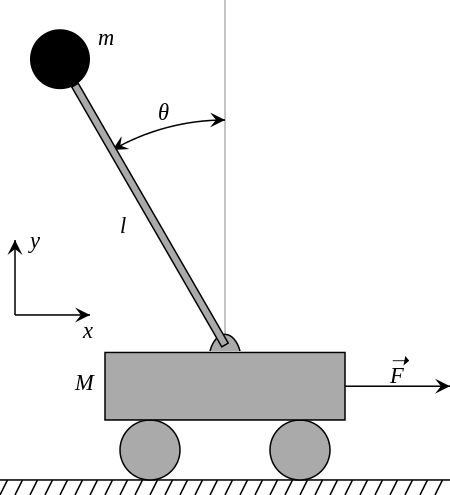
\includegraphics[width=0.6\textwidth]{450px-Cart-pendulum.png}
    \caption{Inverted Pendulum tied to a cart}
    \label{fig:my_label}
\end{figure}
Now we formulate the problem in classical mechanics and reinforcement learning terminology.
We choose the length of the rod $L = 0.5 m$, the mass of the cart $M=1 kg$, the mass of the ball $m=0.1 kg$
and there is no friction between the cart and the floor.
The state of the system is described by
$(x, \theta, \dot{x}, \dot{\theta})$. Notice that $(x, \dot{x})$ is the position of velocity of the cart while
$(\theta, \dot{\theta})$ is the relative position and angular velocity of the ball with respect to the cart.

The action we can do is applying a force
$F$ or $-F$. We specify that the right direction is positive. To make the problem concrete,
we require $F=10N$ and we discrete the time such that at time $t+\Delta t$ we can choose another action.
$\Delta t = 0.02s$. The new state $(x', \theta', \dot{x}', \dot{\theta}')$ is updated from the old state by the following law:
\begin{align*}
x' &= x + \Delta t \cdot \dot{x} \\
\theta' &= \theta + \Delta t \cdot \dot{\theta} \\
\dot{x}' &= \dot{x} + \Delta t \cdot \ddot{x} \\
\dot{\theta}' &= \dot{\theta} + \Delta t \cdot \ddot{\theta}
\end{align*}
The acceleration $(\ddot{x}, \ddot{\theta})$ can be computed from Newton's law.
We list its equation here for convenience:
\begin{align*}
& (m + M)\ddot{x} + mL(\dot{\theta}^2 \sin \theta - \ddot{\theta} \cos \theta) = F \\
& g \sin \theta  + \ddot{x} \cos\theta = L \ddot{\theta}\\
\end{align*}
% check https://en.wikipedia.org/wiki/Inverted_pendulum#Equations_of_motion
There is a reward $r=+1$ for every step taken.

We also set the termination condition when $|\theta| > \delta' \theta = 45^\circ$ and $|x| > \delta x = 4.8 m $.

		
	\end{questions}
	
	
	\nocite{*}
	\begin{flushleft}
		\textbf{Notice}: \\
		\begin{enumerate}
			\item Use matrix operations other than loops for efficiency. If the running time of Auto-Grading steps exceeds 5 minutes, you will get point deductions.
			\item You are expected to only use \texttt{numpy} packages to implement the algorithms.
			\item All questions assume that the data are centered around zero. Therefore, you do not need to train the extra bias parameter in your code.
		\end{enumerate}
	\end{flushleft}
	
	%\bibliographystyle{plain}
	%\bibliography{ref}
	%\begin{thebibliography}{9}
	%	\bibitem{ridge} \href{https://ncss-wpengine.netdna-ssl.com/wp-content/themes/ncss/pdf/Procedures/NCSS/Ridge_Regression.pdf}{Ridge Regression}
	%	\bibitem{tutorial} \href{https://www.datacamp.com/community/tutorials/tutorial-ridge-lasso-elastic-net}{Regularization: Ridge, Lasso and Elastic Net}
	%\end{thebibliography}
\end{document}